\chapter{Question 5 - Extended and Unscented Kalman Filter}
\assignment{
  \begin{enumerate}
    \item When is this estimation methods needed?
    \item What are the differences in theory and practice?
  \end{enumerate}
}

See question 7 for equations

\assignment{1. When is this estimation methods needed?}
\textbf{luenberger observer:} Linear system \\
\textbf{Kalman filter:} Cases where the system can be linearised(once) nicely for the entire desired set \\
\textbf{Extended Kalman filter:} The EKF is good for non-linear systems, where a big span is needed, but no one linearisation can cover the span nicely. \\
\begin{figure}[H]
        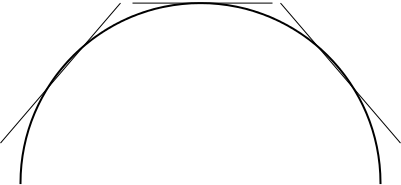
\includegraphics[width=5cm]{EKFsys.png}
\end{figure}
\textbf{Unscented Kalman filter:} The UKF is like the EKF needed for system which cannot be linearised for the entire span nicely. UKF is especially suited for system which is sporadic, and the local linearisation is insufficient.
\begin{figure}[H]
        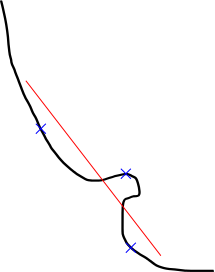
\includegraphics[width=5cm]{UKFsys.png}
\end{figure}

\assignment{2. What are the differences in theory and practice?}
The EKF uses a nonlinear function to estimate the current output based on previous states and control signals. And uses a nonlinear function to predict the next states $\hat{x}_{k+1 \vert k}$
